% DO NOT COMPILE THIS FILE DIRECTLY!
% This is included by the other .tex files.

\begin{frame}[t,plain]
\titlepage
\end{frame}

\begin{frame}
	\frametitle{This session is meant to answer the following}
	\begin{itemize}
		\item (Re-)introduce Cerebrate
                \item Brief summary over the tasks it is meant to accomplish
                \item Cerebrate 1.0 release
                \item Why should MISP users care?
                \item Where are we headed?
                \item Demo time!
	\end{itemize}
\end{frame}

\begin{frame}
	\frametitle{What is Cerebrate?}
	\begin{itemize}
                \item Open source {\bf community management and orchestration} tool
                \item Central tool for the Melicertes 2 project (Co-funded by the EU as a CEF project)
                \begin{itemize}
                    \item Project for the CSIRT network building a common set of tools and services for the national CSIRTs
                \end{itemize}
                \item Tight integration with various open-source tools
                \item Planned as the primary MISP management tool
                \item Test bed for the new tech stack and a host of new features coming to MISP
	\end{itemize}
\end{frame}

\begin{frame}
	\frametitle{Selfish motivations from a MISP perspective}
	\begin{itemize}
            \item {\bf Deficiencies} in our current tool chain
            \begin{itemize}
                \item Do I really have to jump through hoops and long e-mail chains to {\bf onboard new members}?
                \item How do I {\bf find trusted information} on who an organisation is in MISP?
                \item How can I {\bf manage a large cluster of MISPs} without tedious manual labour?
                \item If I run a community through MISP, how can I reuse my member information for other community tasks such as mailing lists?
                \item Information signing has been on the MISP roadmap for a long time - where do we get ground truths for a community from?
            \end{itemize}
        \end{itemize}
\end{frame}

\begin{frame}
	\frametitle{What issues is it trying to tackle?}
	\begin{itemize}
                \item Community management
		\begin{itemize}
                    \item {\bf Repository} of organisations and individuals
                    \item Management of {\bf sharing groups}
                    \item {\bf Exchange} of contact and sharing group information
                    \item Cryptographic key lookup for {\bf information signing}
		\end{itemize}
                \item Local tool management
		\begin{itemize}
                    \item Instrumentation of {\bf local tool interconnections}
                    \item Local tool {\bf fleet management}
                    \item {\bf Feeding} the local tools with Cerebrate data
                \end{itemize}
	\end{itemize}
\end{frame}


\begin{frame}
\frametitle{Interconnections}
    \begin{center}
        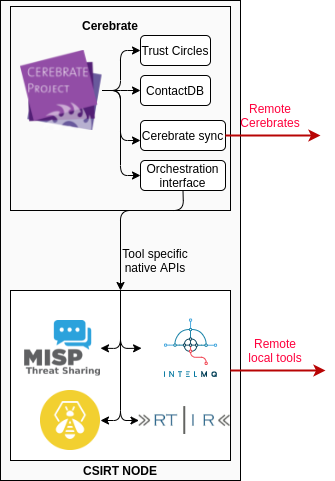
\includegraphics[scale=0.4]{objectives.png}
    \end{center}
\end{frame}

\begin{frame}
	\frametitle{Cerebrate 1.0 release}
	\begin{itemize}
                \item {\bf Released} as October 23
                \item Initial version has the {\bf essential functionalities} to get going included
                \item We highly encourage everyone to {\bf get involved} ASAP and help us mold the tool
                \item {\bf Easy to set up}, low requirements (native or docker installs available)
	\end{itemize}
\end{frame}

\begin{frame}
	\frametitle{Cerebrate 1.0 features}
	\begin{itemize}
            \item {\bf Contact database} \- information on organisations and individuals
            \item {\bf Public key store} for information validation and secure communications
            \item Centralised {\bf sharing group management}
            \item Cerebrate to Cerebrate {\bf synchronisation}
            \item Local integration {\bf module system}
            \item Currently with a {\bf MISP module} included
	\end{itemize}
\end{frame}


\begin{frame}
	\frametitle{Cerebrate 1.0 features}
	\begin{itemize}
            \item Cerebrate to Cerebrate {\bf local tool interconnection}
            \item Local tool {\bf fleet management} features
            \item {\bf Ingestion tools} for community specific {\bf contact database mappings}
            \begin{itemize}
            currently supporting ENISA's and FIRST.org's mappings
            \end{itemize}
            \item Tight integration with {\bf Keycloak} (optional)
	\end{itemize}
\end{frame}

\begin{frame}
\frametitle{MISP to MISP connection request}
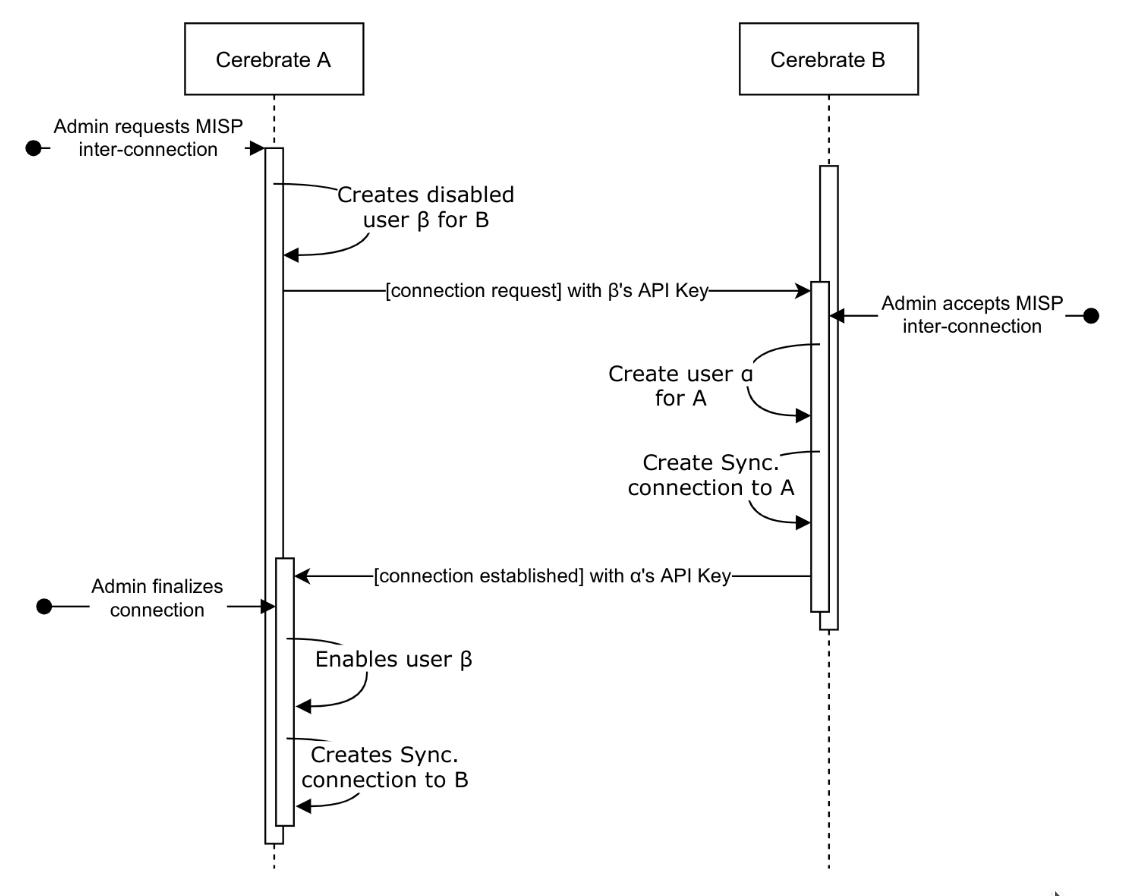
\includegraphics[scale=0.3]{connection_request.png}
\end{frame}

\begin{frame}
\frametitle{MISP to MISP connection request}
    \begin{center}
        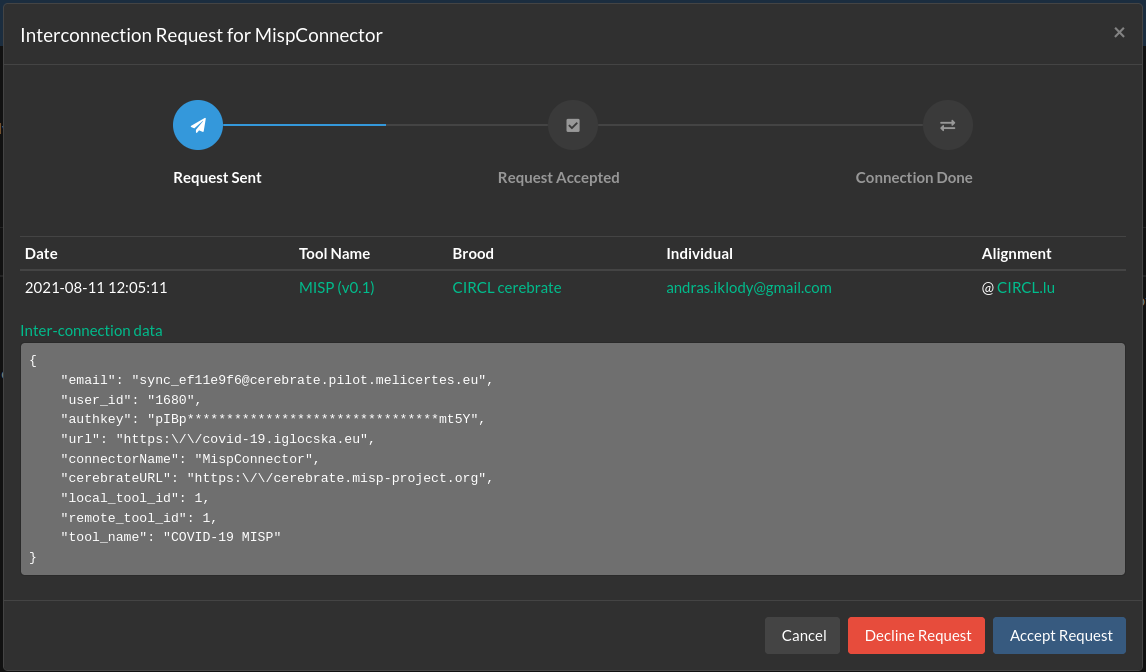
\includegraphics[scale=0.28]{connection_request2.png}
    \end{center}
\end{frame}

\begin{frame}
	\frametitle{Further tangible benefits for MISP}
	\begin{itemize}
            \item MISP's software stack could use a refresher
            \item Cerebrate and MISP share a large part of their code-base and supporting libraries
            \item The similarities in many aspects are no co-incidence
            \item We use Cerebrate to prepare the tooling and gradually shift the MISP code-base to a new stack
            \item CRUD functionalities, UI generation, ACL, API handling are all modernised MISP libraries
	\end{itemize}
\end{frame}

\begin{frame}
	\frametitle{So what will this give MISP once we port it to Cerebrate's codebase?}
	\begin{itemize}
            \item {\bf Modern stack} (CakePHP 4.x, PHP7.4/8+, Bootstrap 5)
            \item Better {\bf performance} (in large part due to CakePHP 4.x's database handling improvements)
            \item Complete {\bf new}, modern, responsive, themeable {\bf UI}
            \item A chance to {\bf clean up} a host of {\bf mistakes} we've made over the years
            \item {\bf Reworked} internal {\bf database} (for example much improved indexing)
            \item A new upgrade and configuration system with a host of improvements
	\end{itemize}
\end{frame}

\begin{frame}
	\frametitle{Cerebrate 1.1}
	\begin{itemize}
            \item Release is planned for {\bf next week}
            \item Main new features
            \begin{itemize}
                \item Reworked meta-field system (validation, filtering, etc)
                \item Audit system (port of Jakub Onderka's implementation from MISP)
                \item Mailing list management and instrumentation
                \item Improved organisation self-management
            \end{itemize}
	\end{itemize}
\end{frame}

\begin{frame}
	\frametitle{What are we working on besides that?}
	\begin{itemize}
                \item Obviously moving MISP to the same feature-set / tech stack
                \item Further integrations with other tools
                \item Fleshing out the MISP monitoring and management
                \item Setting up trusted, community centric Cerebrate nodes
                \item Improving a long list of functionalities
	\end{itemize}
\end{frame}

\begin{frame}
	\frametitle{Enough blabla}
	\begin{itemize}
                \item {\bf Demo time!}
	\end{itemize}
\end{frame}
